\section{Preliminary Numerical Experiments}\label{res:prelim}

		When first considering some system, the critical points tend to be a focus of preliminary attention because they play an important role in the overall dynamics of the system. To see why, we introduce the Schwarzian Derivative and a theorem which tells us how the critical orbit can help dtermine the behavior of all orbits.

		\begin{myth}\label{sch}
			Suppose $SF (X) < 0 \ \forall x$ where $SF$ is the Schwarzian Derivative of some function $F$. If $x_0$ is an attracting periodic point for $F$, then either the immediate basin of attraction of $x_0$ extends to $+\infty$ or $-\infty$, or else there is a critical point of $F$ whose orbit is attracted to the orbit of $x_0$\cite{Dev1}.
		\end{myth}

		\begin{mydef}{Schwarzian Derivative\cite{Dev1} }
		The Schwarzian Derivative of a function $F$ is given by:
		\[
			SF (x) = \frac{F''' (x)}{F' (x)} - \frac{3}{2} \left (\frac{F'' (x)}{F' (x)}\right)^2
		\]
		\end{mydef}

		Thus if an attracting periodic point exists, then the orbit of the critical point will tend toward that periodic point. The only restriction of this theorem is that $F$ must have a negative Schwarzian Derivative, a requirement that our function satisfies as we see below.

		\begin{myprop}
			The function $\ds f_{c, \beta} (x) = x^2 + c + \frac{\beta}{c^2}$ has a negative Schwarzian Derivative for $\beta \geq 0$.
		\end{myprop}

		\begin{myproof}
			Computing the Schwarzian Derivative of our function $f$ we see that 
			\[
				SF (x) = \frac{\frac{\partial^3}{\partial x} \left (x^2 + c + \frac{\beta}{c^2}\right)}{\frac{\partial}{\partial x} \left (x^2 + c + \frac{\beta}{c^2}\right)} - \frac{3}{2} \left (\frac{\frac{\partial^2}{\partial x} \left (x^2 + c + \frac{\beta}{c^2}\right)}{\frac{\partial}{\partial x} \left (x^2 + c + \frac{\beta}{c^2}\right)}\right)^2 = -\frac{24 \beta x^2}{\left (\beta-x^4\right)^2}-\frac{3}{2 x^2}
			\]
			Thus, if beta is positive or 0, each term is positive because every $x$ is raised to an even power. Therefore we have the subtraction of two positive terms so we can conclude that $\forall x$, $SF (x) < 0$.
		\end{myproof}

		Therefore our function has a negative Schwarzian Derivative for $\beta \geq 0$ so an analysis of the critical point (s) should provide a classification of all attracting points in the system. First we compute the critical points of our system:

		\begin{myprop}\label{critp}
			The function $f_{c, \beta} (x) = x^2 + c + \frac{\beta}{x^2}$ has a critical point at each $\pm \beta^{\frac{1}{4}}$.
		\end{myprop}

		\begin{myproof}
			The critical points of a function are defined to be the points with slope 0. Solving we find that:
			\[
			F_c' (x) = 0  \Ra 2x - \frac{2\beta}{x^3} = 0 \Ra 2x = \frac{2\beta}{x^3} \Ra x = \pm\beta^{\frac{1}{4}}
			\]
		\end{myproof}

		Thus we have two critical points in the real setting, however when we plug these points into our system we see that:
		\[
			f_{c, \beta} (\beta^{\frac{1}{4}}) = \left (\beta^{\frac{1}{4}}\right)^2 + c + \frac{\beta}{\left (\beta^{\frac{1}{4}}\right)^2} = 2 \beta^{\frac{1}{2}} + c = \left (-\beta^{\frac{1}{4}}\right)^2 + c + \frac{\beta}{\left (-\beta^{\frac{1}{4}}\right)^2} = f_{c, \beta} (-\beta^{\frac{1}{4}})
		\]
		Thus, while we have two critical points, we really only have one critical value such that the orbits of $\pm \beta^{\frac{1}{4}}$ vary only by the zeroeth iterate.

		\begin{figure}[h]
			\centering
			\begin{subfigure}[b]{0.5\textwidth}
					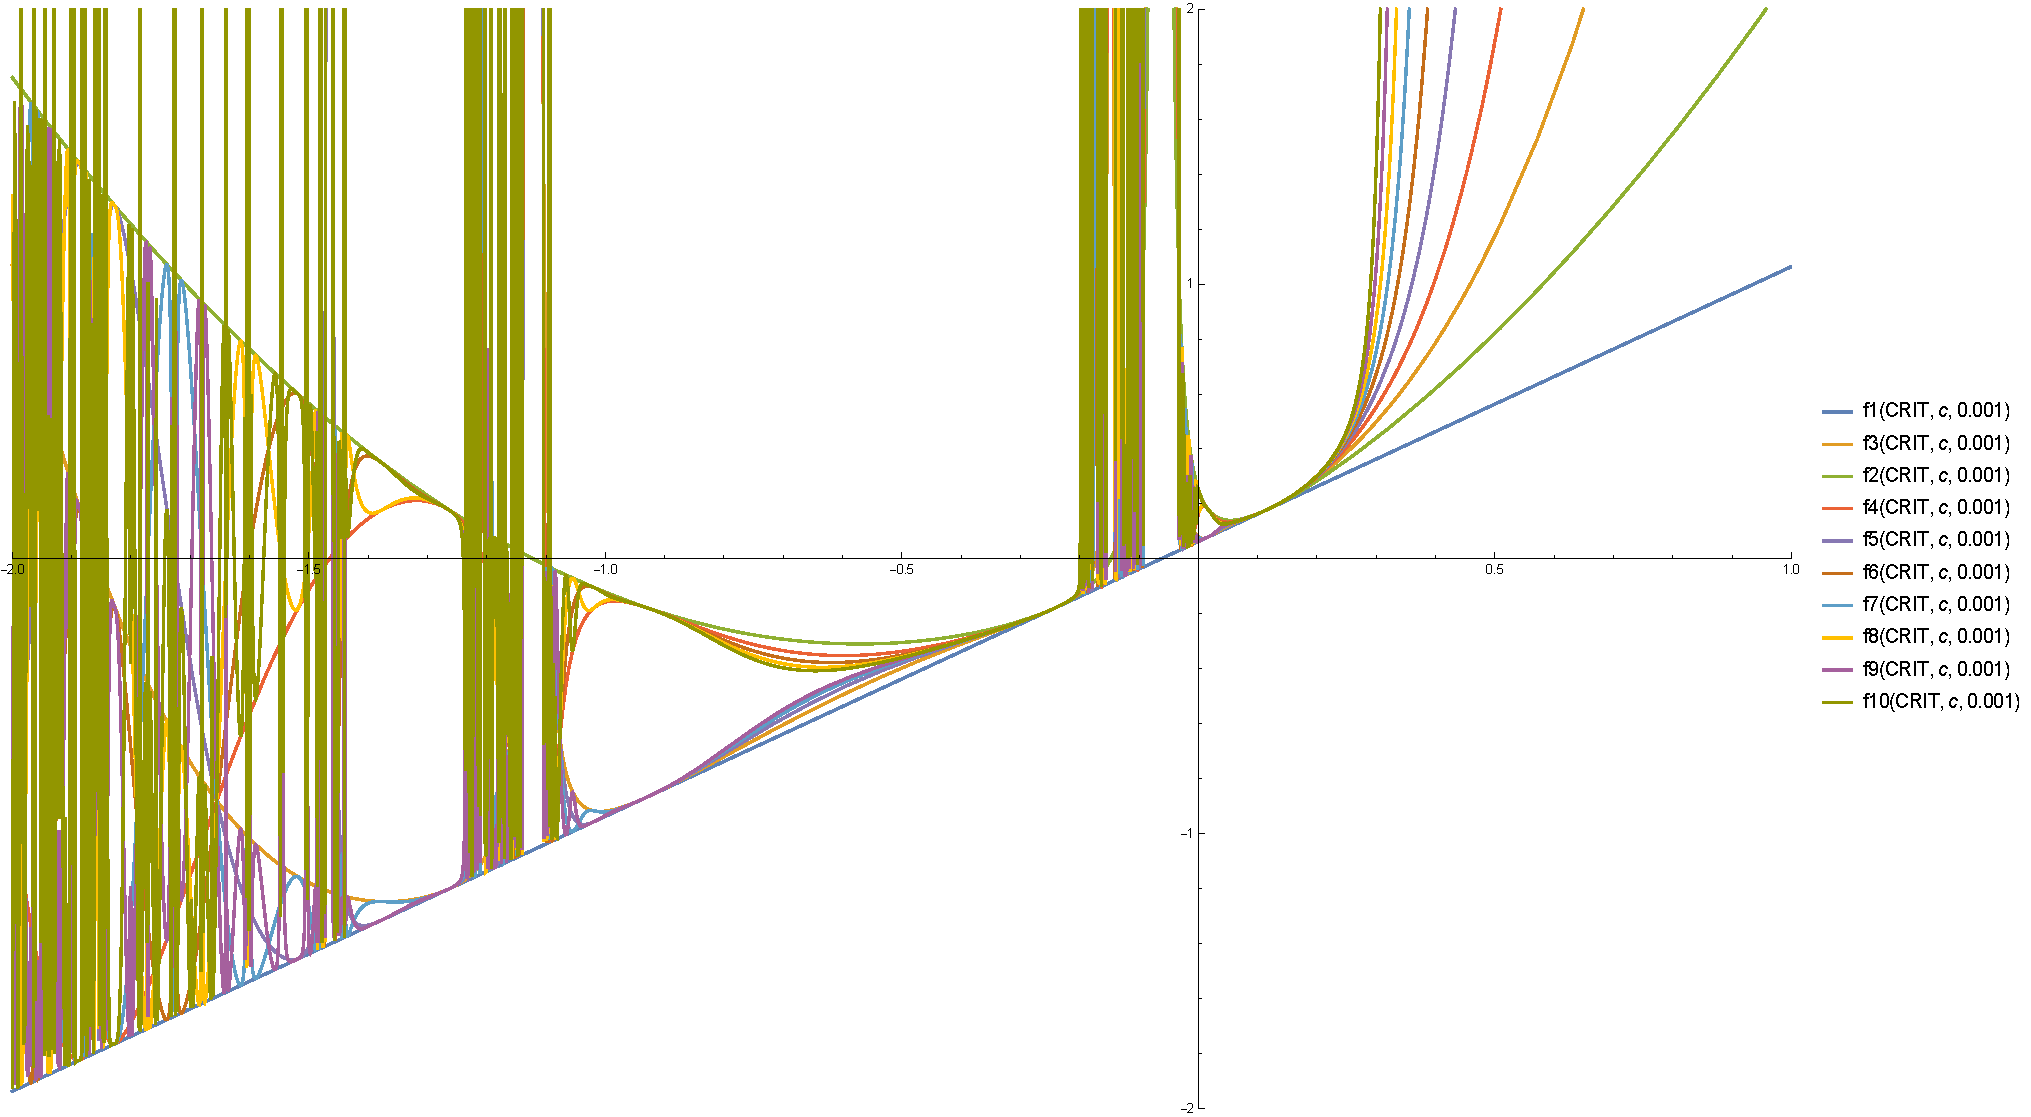
\includegraphics[width=\textwidth]{pert}
					\caption{Orbit diagram of $x^2 + c + \frac{.001}{x^2}$}
					\label{pert}
			\end{subfigure}%
			\begin{subfigure}[b]{0.5\textwidth}
					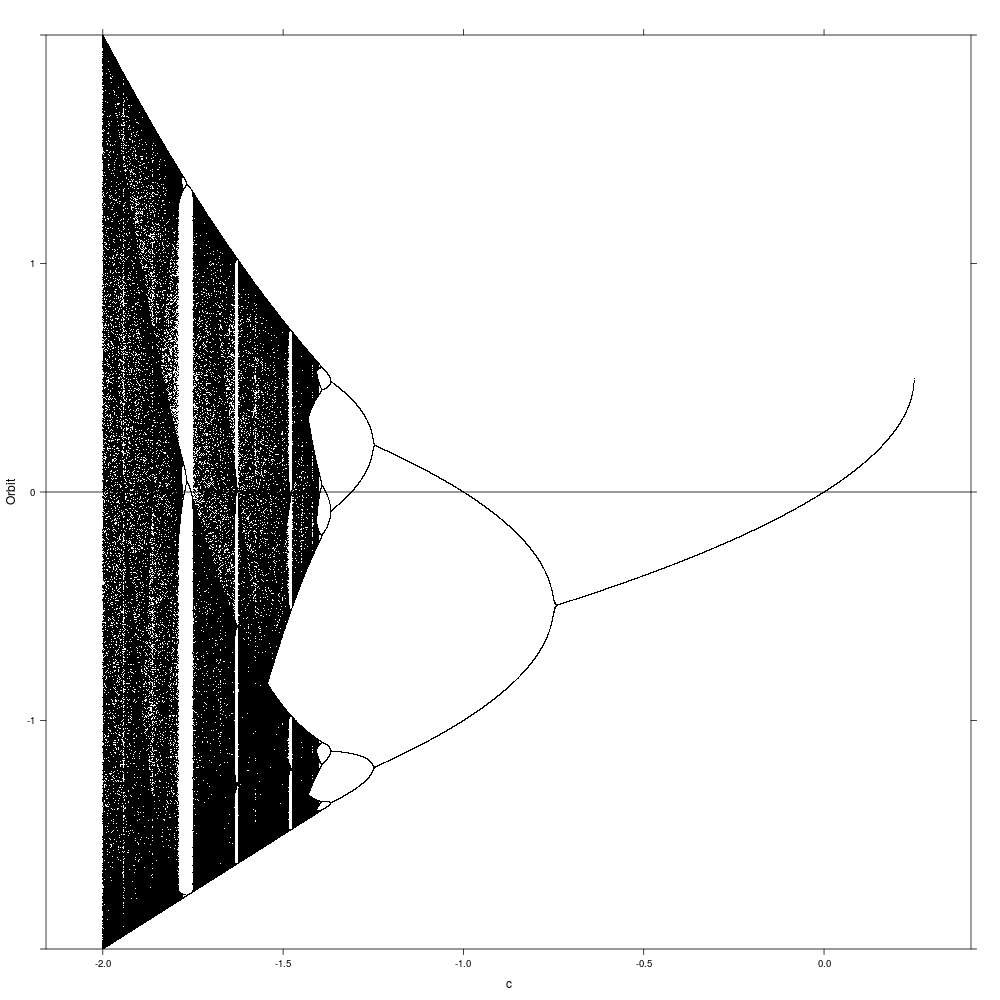
\includegraphics[width=\textwidth]{orig}
					\caption{Orbit diagram of $x^2 + c$}
					\label{stand}%
			\end{subfigure}
			\caption{Orbit diagrams of the original system and the perturbed system}\label{fig:orbits}
		\end{figure}

		Now that we have established that the behavior of the critical point helps determine the behavior of the system, we can perform a few numerical experiments to discover where the perturbed system varies from the original quadratic map. A standard analysis of the behavior of the critical point is to create an orbit diagram as shown in Figure \ref{pert} and Figure \ref{stand}. Immediately we can see some major differences between the behavior of the two families. One of the most notable differences is on the parameter interval $c\in (-.25, .05)$, a magnification of which is shown in Figures \ref{pertz2} and \ref{pertz1}.

		The following section will discuss the behavior of the system for $c$ intervals which are either straightforward or analogous to the behavior of the original quadratic map. Subsequent sections will then describe some of the behavior where the perturbed  map acts quite differently than the standard map, proving some instances of interesting critical orbit behavior.

		\begin{figure}[h]
			\centering
			\begin{subfigure}[b]{0.5\textwidth}
					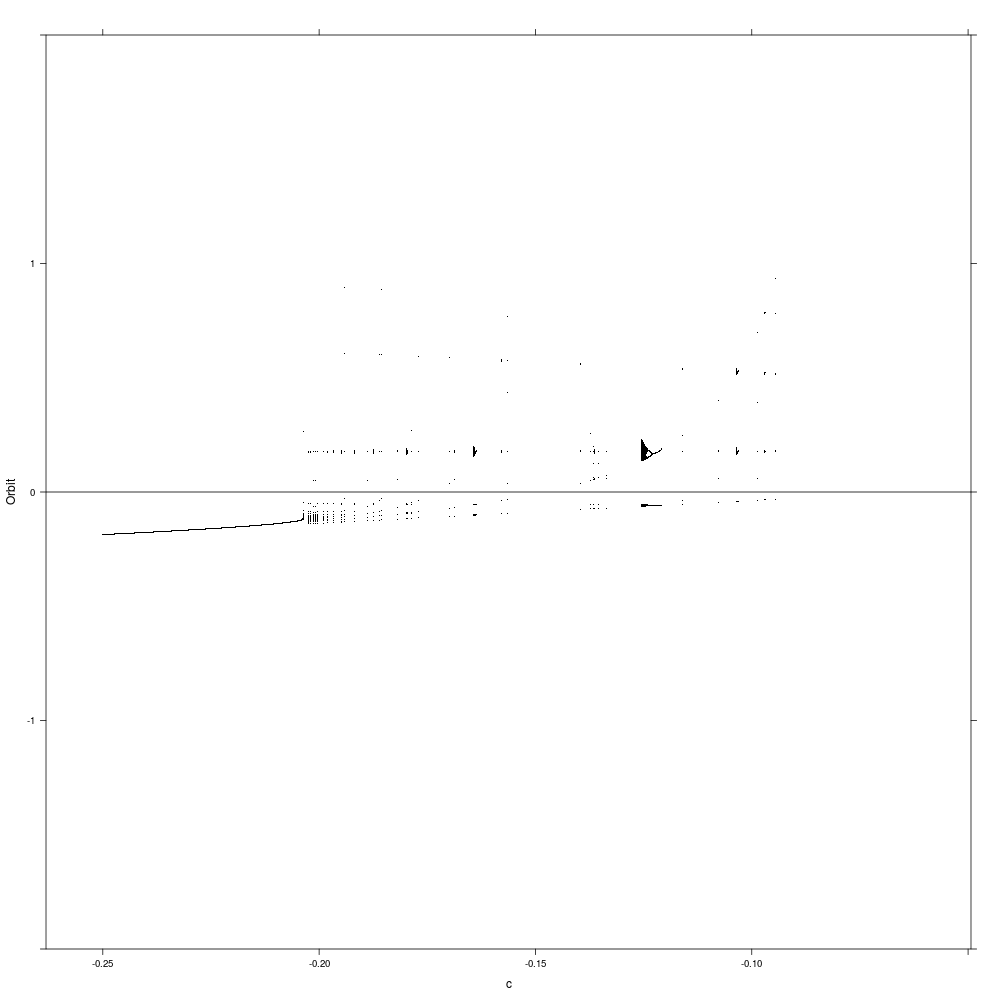
\includegraphics[width=\textwidth]{pertzoom2}
					\caption{$c\in (-.25, .062456)$}
					\label{pertz2}
			\end{subfigure}%
			\begin{subfigure}[b]{0.5\textwidth}
					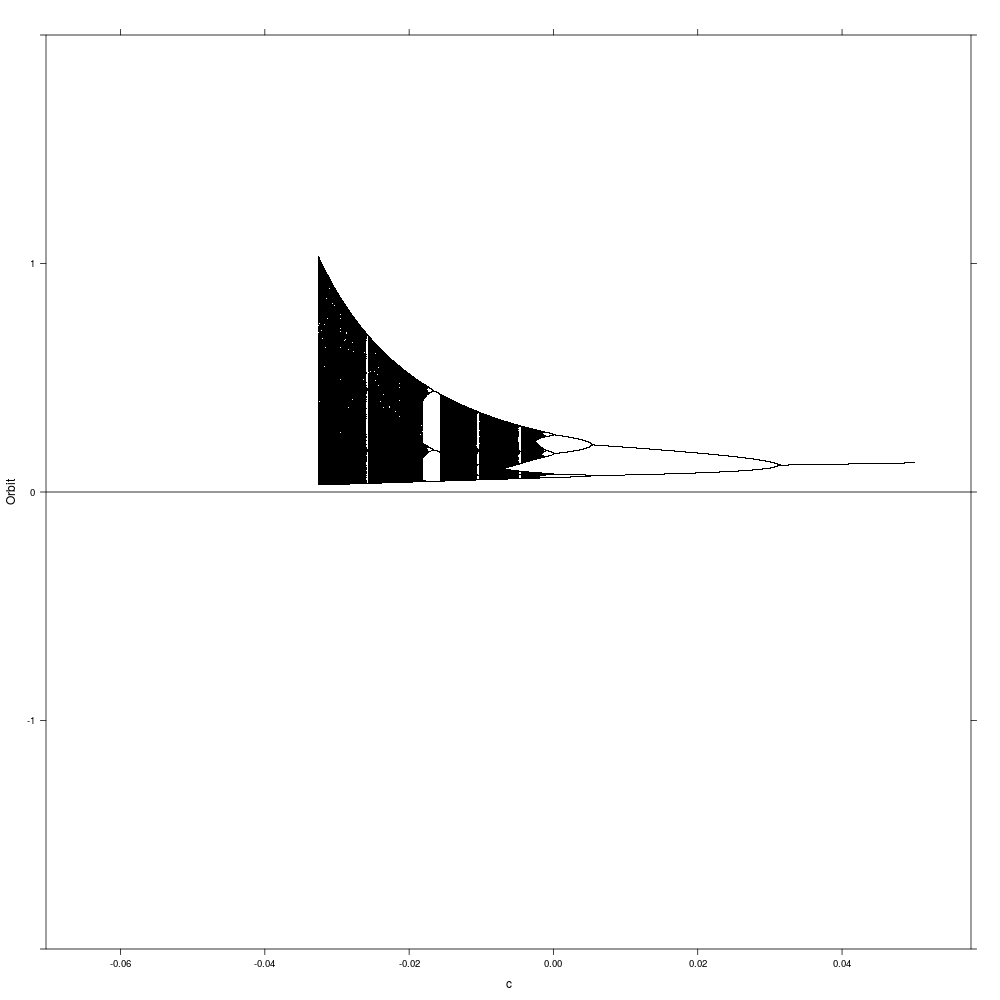
\includegraphics[width=\textwidth]{pertzoom1}
					\caption{$c\in (-.062456, .05)$}
					\label{pertz1}%
			\end{subfigure}
			\caption{Orbit diagrams of the original system and the perturbed system}\label{fig:orbits2}
		\end{figure}